% ++++++++++++++++++++++++++++++++++++++++
% Don't modify this section unless you know what you're doing!
\documentclass[letterpaper,12pt]{article}
\usepackage{tabularx} % extra features for tabular environment
\usepackage{amsmath}  % improve math presentation
\usepackage{graphicx} % takes care of graphic including machinery
\usepackage[margin=0.75in,letterpaper]{geometry} % decreases margins
\usepackage{cite} % takes care of citations
\usepackage[final]{hyperref} % adds hyper links inside the generated pdf file
\usepackage{listings}
\usepackage{csvsimple}
\usepackage{verbatim}
\usepackage{float}
\usepackage{graphicx} % Allows including images
\hypersetup{
	colorlinks=true,       % false: boxed links; true: colored links
	linkcolor=black,        % color of internal links
	citecolor=blue,        % color of links to bibliography
	filecolor=magenta,     % color of file links
	urlcolor=blue         
}
%++++++++++++++++++++++++++++++++++++++++
\setlength{\parindent}{0pt}
\setlength\parskip{1em plus 0.1em minus 0.2em}

\begin{document}
\title{%
PyLab - SpringMass \\
\large PHY224 Lab 3}
\author{Fredrik Dahl Bråten, Pankaj Patil}
\date{\today}
\maketitle
%\tableofcontents
%\listoffigures
%\listoftables

\section{Abstract}

In this exercise, we studied the equation of motion of a mass-spring system in damped and undamped 
cases. In both the cases the we verified the experimental data with that obtained using qualitative 
fit of equation of motion. This analysis was done in Python by use of the numpy, scipy and matplotlib modules.

\section{Introduction}

The undamped spring mass equation is given by the Hook's law, 
$$F_{spring} = -ky$$
Where $y$ is the vertical displacement of the mass and $k$ is the spring constant.
Above equation is used to derive the equation of motion of  the spring mass system,
\begin{equation}
  \frac{d^2y}{dt^2} + \Omega_{0}^2y = 0 \implies y = y_0 + A\sin(\Omega_0 t)
\end{equation}
Where $\Omega_0 = \sqrt{\frac{k}{m}},\ A = \text{Amplitude of Oscillations},\ y_0 = \text{Initial Position of the mass}$

In case of damping, we need to add damping force to the equation which depends on the velocity of the mass relative
to surrounding medium. In our case, where we have small Reynolds numbers, the drag force is directly proportional
to the velocity of the mass,
$$\vec{F_d} = -\gamma \vec{v} $$
Where $\gamma$ is damping coefficient. The equation of motion is then given by

\begin{equation}
  \frac{d^2y}{dt^2} + \gamma\frac{dy}{dt} + \Omega_{0}^2y = 0 \implies y = y_0 + A e^{-\gamma t}\sin(\Omega_0 t) 
\end{equation}

In both the cases, we qualitatively fit the data to the above displacement equations.

\section{Methods, Materials and Experimental Procedure}

We successfully followed the procedures as described by the TA for this experiment.

\section{Results}
\subsection{Undamped Spring Mass}

In Appendix Figure \ref{undamped-plot}, we see the displacement data is 
plotted against time for the undamped case. The graph is a qualitative fit 
of the equation describing the undamped oscillatory motion of spring-mass system.

Using the qualitative fit we obtained following values,
\begin{itemize}
  \item[] $y_0=$ Initial Position = 20.71 $cm$
  \item[] $A=$ Amplitude = 0.70 $cm$
  \item[] $\Omega_0=$ Frequency of Oscillations = 9.07 $rad/s$
\end{itemize}

Using the $\Omega_0$ value we obtain the spring constant $$k = m \Omega^2_0 = 16.44\ kg/s^2$$

The simulated data for the undamped case is plotted in Figure \ref{undamped-sim-plot}. 

\subsection{Damped Spring Mass}

In Appendix Figure \ref{damped-plot}, we see the displacement data is 
plotted against time for the damped case. The graph is a qualitative fit 
of the equation describing the damped oscillatory motion of spring-mass system.

Using the qualitative fit we obtained following values,
\begin{itemize}
  \item[] $y_0=$ Initial Position = 19.94 $cm$
  \item[] $A=$ Amplitude = 1.64 $cm$
  \item[] $\gamma=$ Damping Coefficient = 0.01
  \item[] $\Omega_0=$ Frequency of Oscillations = 8.69 $rad/s$
\end{itemize}

Using the $\Omega_0$ value we obtain the spring constant $$k = m \Omega^2_0 = 16.24\ kg/s^2$$

The simulated data for the damped case is plotted in Figure \ref{damped-sim-plot}. 

\section{Discussion}

For the undamped spring-mass system,

\begin{itemize}
  \item[] $F_{spring} = -ky$ \ \ \ \ \ Hook's Law
  \item[] $F=ma$ \ \ \ \ \ \ \ \ \ \ \ \ \ Newton's Second Law of Motion
  \item[] $\implies ma = -ky$ 
  \item[] $\implies m\frac{d^2y}{dt^2} = -ky$
  \item[] $\implies m\frac{d^2y}{dt^2} + ky = 0$
\end{itemize}

We approximated that the motion of the system is purely one dimensional in only y-direction.

The equation of motion can be written as,
\begin{eqnarray*}
  \begin{split}
    &\frac{d^2y}{dt^2} = -\Omega_0^2 y \ \ \ \ \text{where } \Omega_0 = \sqrt{\frac{k}{m}} \\
    \implies &\frac{dv}{dy} = -\Omega_0^2 y \ \ \ \text{ where } \frac{d^2y}{dt^2} = \frac{dv}{dy},\ \ \ \  v = \frac{dy}{dt} \\
    \implies &\frac{1}{\Delta t} [v(t+\Delta t) - v(t)] =  -\Omega_0^2 y \ \ \ \ \ \text{using Forward Euler method} \\
    \implies &[v(t+\Delta t) - v(t)] =  -\Delta t \Omega_0^2 y\\
    \implies &v(t+\Delta t) =  v(t) -\Delta t \Omega_0^2 y\\
  \end{split}
\end{eqnarray*}
And 
\begin{eqnarray*}
  \begin{split}
    &v = \frac{dy}{dt} \\
    \implies &\frac{1}{\Delta t} [y(t+\Delta t) - y(t)] =  v(t) \ \ \ \ \ \text{using Forward Euler method} \\
    \implies &y(t+\Delta t) =  y(t) + \Delta t v(t)\\
  \end{split}
\end{eqnarray*}

Thus the Forward Euler methods gives us,
\begin{eqnarray*}
  \begin{split}
    y_{i+1} &= y_i + \Delta t v_i \\
    v_{i+1} &= v_i -\Delta t \Omega_0^2 y_i
  \end{split}
\end{eqnarray*}
for $i = 0, 1, 2, \dots$

Above equations were used to compute the simulated oscillation which are plotted in Figure \ref{undamped-sim-plot}. 

The oscillatory motion of spring mass system is a sinusoidal graph, which is expected as it is a periodic motion.

For the undamped spring-mass system, the mechanical energy is conserved and is given by,

$$E_{tot} = \frac{1}{2}mv^2 + \frac{1}{2}ky^2$$

Rearranging above give,

$$\frac{v^2}{k} + \frac{y^2}{m} = \frac{2E_{tot}}{mk}$$

Which is an equation of an ellipse. Hence the phase plot of system is an ellipse.

In damped oscillations, as expected the amplitude of oscillation decays exponentially as os evident
from Figure \ref{damped-plot}.

\section{Conclusions}

By approximating the motion in one dimension, we established that the equation of motion of spring-mass 
system in undamped case is given by Eqn (1). And that for damped system is give by Eqn. (2). In undamped 
system the energy of the system is conserved. Qualitative fit of the solution to equation of motion 
enables us to compute the spring constant, in both the cases and it is found to be in agreement within experimental errors.
The qualitative fit establishes that the motion of spring-mass system is sinusoidal with constant period. In 
case of damping the amplitude of the motion decays exponentially.

\pagebreak

\appendix

\section{Appendix}

\subsection{Plots For Undamped Spring-Mass  System}
\begin{figure}[H]
  \centering
  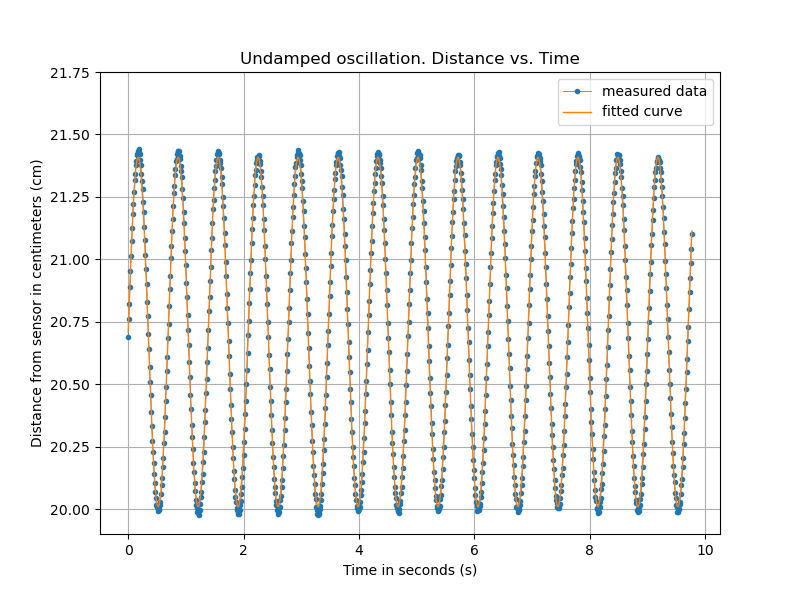
\includegraphics[width=0.95\linewidth]{../Fredrik/Undamped oscillation. Distance vs. Time.png}    
  \begin{center}
    \emph{}
  \end{center}
  \caption{Undamped Oscillations}
  \label{undamped-plot}
\end{figure}

\begin{figure}[H]
  \centering
  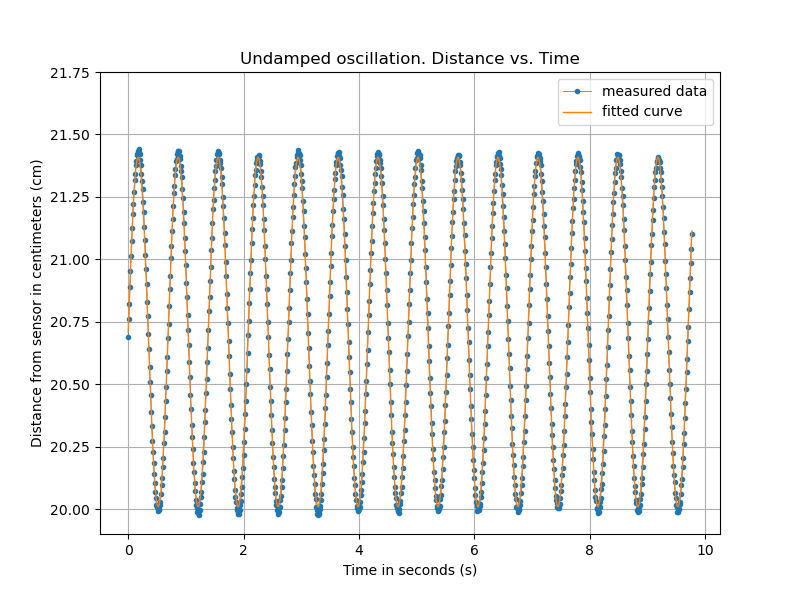
\includegraphics[width=0.95\linewidth]{../Fredrik/Undamped oscillation. Distance vs. Time.png}    
  \begin{center}
    \emph{}
  \end{center}
  \caption{Undamped Oscillations}
  \label{undamped-sim-plot}
\end{figure}

\subsection{Plots For Damped Spring-Mass  System}
\begin{figure}[H]
  \centering
  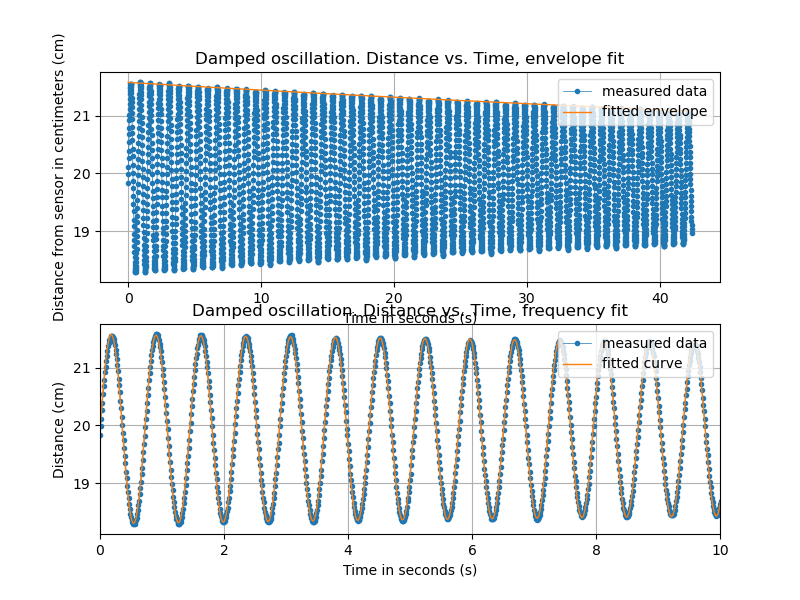
\includegraphics[width=0.95\linewidth]{../Fredrik/Damped oscillation. Distance vs. Time.png}    
  \begin{center}
    \emph{}
  \end{center}
  \caption{Damped Oscillations}
  \label{damped-plot}
\end{figure}

\begin{figure}[H]
  \centering
  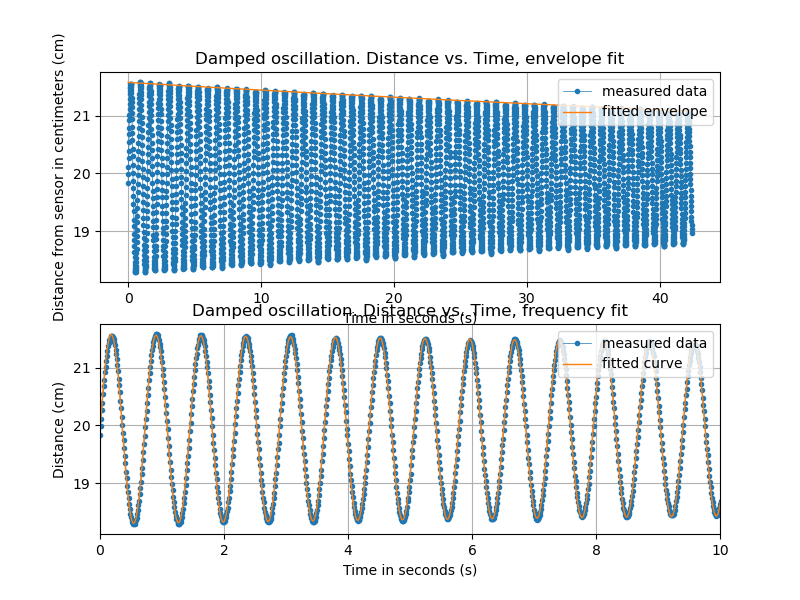
\includegraphics[width=0.95\linewidth]{../Fredrik/Damped oscillation. Distance vs. Time.png}    
  \begin{center}
    \emph{}
  \end{center}
  \caption{Damped Oscillations}
  \label{damped-sim-plot}
\end{figure}

\pagebreak

\subsection{Python Code}

The Python code for this exercise is divided into two files. Functions.py file contains utility methods
which we will be frequently using in this course. Undamped\_and\_Damped.py file contains the code which analyzes
the data.

\subsubsection{Functions.py}
\noindent\rule{\textwidth}{1pt}
\verbatiminput{../Fredrik/Functions.py}
\noindent\rule{\textwidth}{1pt}

\subsubsection{Functions.py}
\noindent\rule{\textwidth}{1pt}
\verbatiminput{../Fredrik/Undamped_and_Damped.py}
\noindent\rule{\textwidth}{1pt}

\begin{thebibliography}{99}

\bibitem{lab-manual-ex4} Lab Manual - Spring Mass - exercise4\_NI.pdf

\end{thebibliography}

\end{document}
